\documentclass[11pt]{article}

\usepackage{iftex}
\ifPDFTeX
  \usepackage[T1]{fontenc}
  \usepackage[utf8]{inputenc}
  \usepackage{lmodern}
\fi
\usepackage[letterpaper,margin=1in]{geometry}
\usepackage{amsmath,amssymb,amsthm}
\usepackage{booktabs,tabularx,array,longtable}
\usepackage{enumitem}
\usepackage{xcolor}
\usepackage{tikz}
\usetikzlibrary{positioning,arrows.meta,fit,calc,shapes.geometric,backgrounds}
\usepackage[numbers,sort&compress]{natbib}
\usepackage{xurl}
\usepackage[hidelinks]{hyperref}
\usepackage{microtype}
\usepackage{caption}

\setlist{itemsep=2pt,topsep=4pt}
\setlength{\emergencystretch}{3em}
\captionsetup{font=small,labelfont=bf}

\newtheorem{property}{Property}
\theoremstyle{definition}
\newtheorem{assumption}{Assumption}

\newcommand{\code}[1]{\texttt{\small #1}}
\newcommand{\Hash}{\mathsf{H}}
\newcommand{\tx}[1]{\mathsf{tx}_{\mathrm{#1}}}

\title{OpenBazaar: Signed Catalogs, Sealed Orders, and\\Scriptless Two-Party Escrow for a Non-Custodial Marketplace}
\author{Brian Hoffman\\[2pt]\normalsize OpenBazaar project}
\date{November 2026}

\begin{document}
\maketitle

\begin{abstract}
OpenBazaar is a peer-to-peer marketplace for ordinary physical and digital goods paid in bitcoin. The original system (developed from 2014, with its last substantial releases in 2020) published stores over IPFS, carried orders over libp2p, and protected buyers with a 2-of-3 multisignature escrow whose script and moderator key appeared on chain when it was spent. This paper describes a redesign and argues which of its security and privacy properties hold, under which assumptions, and how much of each is implemented today.

Stores and listings are public, content-addressed records signed with BIP 340 Schnorr signatures over a canonical encoding. Orders are private letters sealed with HPKE to a single vendor and addressed to that vendor's onion-service mailbox; a client device talks only to its owner's node. Payments go directly to the vendor, one transaction per seller. Moderated purchases use a scriptless escrow: a MuSig2 Taproot key-path output whose timeout and dispute spends are all presigned before funding. A dispute is settled by an adaptor signature whose completing secret is split between the favored party and a moderator half that the losing party verifiably encrypts to the moderator. The moderator never holds a signing key over the funds and cannot change any payout.

We state the threat model, give the escrow protocol and its timeline precisely, tabulate what every observer learns, and label each mechanism as implemented and tested, implemented as a demonstration, specified but not implemented, or future work. At the time of writing, live Tor delivery, catalog replication, publishing costs, and integration of the two-party escrow into the node are not implemented, and the paper's analysis of those parts is a design argument rather than a description of running code.
\end{abstract}

\section{Introduction}
\label{sec:intro}

A marketplace has to do four things: let sellers publish what they offer, let buyers find it, carry an order from buyer to seller, and settle payment in a way both sides can accept. Hosted marketplaces do all four in one place. That place can see every order, hold every payment, and remove any seller. OpenBazaar's premise is that these functions can be split so that no single operator is needed for any of them, and so that the parties who must learn something (the seller who ships, the moderator who rules on a dispute) learn it only when they need to.

\subsection{The original OpenBazaar}

OpenBazaar began in 2014 as a prototype peer-to-peer market and was developed as \code{openbazaar-go} and a desktop client until late 2020~\citep{openbazaargo}. A node published its store as an IPFS directory addressed by IPNS~\citep{ipfs}. Listings were signed by the node's identity key. Messages traveled over libp2p when both peers were online; when the recipient was offline, the sender stored the message on its own node or an external storage host and left a pointer in the distributed hash table. Search was a separate hosted index that nodes notified on publish. The wallet supported several cryptocurrencies. Moderated purchases used a 2-of-3 multisignature script over buyer, vendor, and moderator keys, with a default timeout of 1080 hours.

That design had strengths the redesign keeps: listings were signed and an order committed to a hash of the listing it bought, so later edits could not rewrite a deal; the moderator could not take funds alone. It also had properties the redesign changes:
\begin{itemize}
  \item A store was available only while its own node, or a pinning service, was online.
  \item The libp2p peer identity was long-lived and observable, and peers dialed each other directly, so the network layer linked a store identity to IP addresses.
  \item The default search index was a single hosted service. Delisting from it removed a store from practical discovery.
  \item Spending a 2-of-3 P2SH or P2WSH output reveals the full script, including the moderator's public key, so every moderated purchase was recognizable on chain and attributable to its moderator.
  \item A phone could not run the daemon in the background, so a vendor without an always-on desktop missed orders.
  \item The multi-coin wallet made wallet maintenance the dominant engineering cost.
\end{itemize}

\subsection{This paper}

The redesign keeps the contract between buyer, vendor, and moderator and replaces the machinery underneath. Its main ideas are:
\begin{enumerate}
  \item \textbf{A public catalog, private orders.} Store and listing records are public, signed, and content-addressed, and replicated by any node (\S\ref{sec:catalog}). Orders are not catalog records; each is a letter sealed to one vendor and carried to that vendor's own mailbox (\S\ref{sec:orders}). Vendors label their own records, and buyers filter what they see on their own devices (\S\ref{sec:labels}).
  \item \textbf{Clients that only talk to their own node.} The user-facing app sends marketplace requests to its owner's node, which verifies records and delivers letters (\S\ref{sec:architecture}). A phone reaches that node as in \S\ref{sec:remote}.
  \item \textbf{Direct, per-seller payments.} A buyer pays each vendor in a separate transaction, never batching two sellers together (\S\ref{sec:payments}).
  \item \textbf{Scriptless two-party escrow with a bounded moderator.} The escrow output is an ordinary-looking Taproot key-path output. Every non-cooperative outcome is presigned by both parties before the buyer funds it. The moderator only reveals one secret scalar that completes one of two presigned dispute outcomes (\S\ref{sec:escrow}).
\end{enumerate}

The contributions are: (i) a threat model for a marketplace with this split (\S\ref{sec:threats}); (ii) a precise description of the two-party escrow protocol, its message rounds, the checks each party and the moderator must run, and its block-height timeline (\S\ref{sec:escrow}); (iii) argued security properties, each with its assumptions, and the attacks the checks exist to stop (\S\ref{sec:security}); (iv) a table of what every party and observer learns (\S\ref{sec:privacy}); and (v) measurements of a reference implementation (\S\ref{sec:evaluation}) and a statement of what the design does not achieve (\S\ref{sec:limitations}).

A reference implementation in Rust, with a web and desktop client and a native phone app for iOS and Android, is available at \url{https://github.com/OpenBazaar/openbazaar-rs}. This paper describes what that implementation does.

\section{Design Goals and Non-Goals}
\label{sec:goals}

\subsection{Goals}

\begin{description}[leftmargin=1.2em]
  \item[G1. No custody.] No party other than the buyer and the vendor ever holds a key, or a set of keys, sufficient to move a buyer's payment. The moderator in particular holds no signing key over escrowed funds.
  \item[G2. Verifiable public catalog.] Anyone can check that a listing was published by the store it names and has not been altered. A listing's address is derived from its content.
  \item[G3. Private orders.] An order's contents, including any ship-to address, are readable only by the vendor it is addressed to. No public relay or index stores a record that a given buyer wrote to a given vendor.
  \item[G4. Bounded moderation.] A moderator can choose between two payouts that buyer and vendor already signed. It cannot sign alone, redirect funds, change amounts, or learn about an order unless a party opens a dispute.
  \item[G5. Liveness without a platform.] A buyer can recover escrowed funds from a vendor who disappears, and a vendor can collect from a buyer who stops responding, without anyone's cooperation beyond broadcasting a presigned transaction.
  \item[G6. Thin clients.] A phone client embeds Tor so it can reach the node it is paired with. It does not hold spend keys, and it does not dial other vendors. A browser on the same machine talks to the node on a loopback address. Spending and chain watches stay on the node.
  \item[G7. Honest degradation.] When a privacy mechanism is unavailable (no Tor, no Payjoin partner, no Lightning route), the system says so rather than silently falling back.
\end{description}

\subsection{Non-goals}

\begin{itemize}
  \item \textbf{Anonymity against a global passive adversary.} We do not claim unlinkability against an adversary that observes most of the network. Section~\ref{sec:privacy} states what such an adversary learns.
  \item \textbf{Hiding the catalog.} Listings are public by design. A market that cannot be discovered does not serve its purpose.
  \item \textbf{Hiding the ship-to address from the seller or the carrier.} A seller of a physical good must learn where to send it, and the carrier must deliver it. This is a ceiling on buyer privacy for physical goods, not a gap to be engineered away.
  \item \textbf{Deciding factual disputes cryptographically.} Whether a parcel contained the right item is a judgment by a person. The protocol bounds what that person can do with the funds; it does not replace the judgment.
  \item \textbf{Reputation.} A review or rating system is outside this paper.
  \item \textbf{Content policy.} The protocol is designed for ordinary goods. Policies for what may be listed, and the obligations of people who operate replicas or seeds, are outside the scope of this paper.
\end{itemize}

\section{System Model and Actors}
\label{sec:model}

\paragraph{Devices.} A \emph{client} is the user-facing application: an installed web app on a phone, or the same screens inside a desktop shell. A \emph{node} is a long-running process the user controls, on a desktop computer or an Android device, that holds keys, stores records, talks to the network, and watches the Bitcoin chain. A client is paired with exactly one node. In the intended deployment the phone has no Tor client and never dials the peer-to-peer network; it talks only to its paired node and stops working when that node is unreachable \SP. Today the client and node run on the same machine and talk over loopback HTTP \IT.

\paragraph{Roles.}
\begin{description}[leftmargin=1.2em]
  \item[Buyer.] Browses the catalog, sends a sealed order, and pays. For moderated purchases, funds the escrow output and holds a presigned refund.
  \item[Vendor.] Publishes a signed store and listings, runs a node with an onion-service mailbox, opens letters, ships, and collects payment. For moderated purchases, holds a presigned claim.
  \item[Moderator.] Named in a listing and in the signed escrow terms. Receives nothing unless a party opens a dispute. On a dispute, verifies a self-contained letter and reveals one secret scalar to the party it rules for. Paid a fixed fee by the dispute outcome.
  \item[Replica.] A node that stores and serves catalog records it did not create, so that a store remains readable while its publisher is offline \SP.
  \item[Seed.] A node whose address ships with the software or is pasted by the user, used only to find other nodes. Seeds are untrusted for content: every record is verified against its signature \SP.
\end{description}

\paragraph{External parties.} The Bitcoin network and chain; a block-explorer API (Esplora) that the node queries for chain state \IT{} in PR~\#2; Tor relays \SP{} for live use; Lightning routing nodes \SP{} for payment; a public exchange-rate endpoint the node queries for fiat estimates \IT; and, for physical goods, a parcel carrier.

\paragraph{Records and messages.} A \emph{store record} names a store key, a display name, a region, and direct-payment strings. A \emph{listing} names its store key and describes one offer. An \emph{order letter} is an HPKE ciphertext addressed to one vendor. \emph{Escrow messages} are the three funding rounds and the release exchange between buyer and vendor. A \emph{dispute letter} goes from one party to the moderator, and a \emph{ruling} comes back.

\paragraph{Network assumptions.} We assume the Bitcoin chain makes progress and that a transaction paying a sufficient fee rate is confirmed within a bounded number of blocks; the escrow windows in \S\ref{sec:escrow} are sized against this assumption. We do not assume synchronous delivery between buyer and vendor nodes.

\section{Threat Model}
\label{sec:threats}

We consider the adversaries in Table~\ref{tab:adversaries}. For each, we state what it controls and whether defending against it is in scope. ``In scope'' means the design claims a property against that adversary under stated assumptions; ``characterized'' means we describe what the adversary achieves without claiming to prevent it.

\begin{table}[ht]
\centering\small
\begin{tabularx}{\textwidth}{@{}p{0.2\textwidth}Xp{0.14\textwidth}@{}}
\toprule
\textbf{Adversary} & \textbf{Capabilities} & \textbf{Scope} \\
\midrule
A1 Network observer & Sees, delays, and drops traffic on some links (a local network, an ISP, a single Tor relay). & In scope \\
A2 Malicious replica or seed & Serves, withholds, or reorders catalog records; lies about other nodes; logs who fetches what. & In scope for integrity; availability characterized \\
A3 Malicious counterparty & A buyer or vendor who deviates arbitrarily from the protocol, including going silent. & In scope \\
A4 Malicious moderator & Rules dishonestly, rules for both sides, refuses to rule, or logs disputes. & In scope for funds; ruling quality characterized \\
A5 Moderator colluding with one party & The moderator and either the buyer or the vendor act together. & Characterized \\
A6 Compromised device & Reads files or memory on a user's node or client. & Characterized \\
A7 Global passive adversary & Observes most network links and the chain. & Out of scope; characterized \\
\bottomrule
\end{tabularx}
\caption{Adversaries considered.}
\label{tab:adversaries}
\end{table}

A5 is inherent to any escrow with a third-party arbiter: if the arbiter and one party agree, the arbiter can rule for that party. The protocol limits A5 to choosing the presigned outcome that favors the colluding party; it cannot pay a third party or change amounts (\S\ref{sec:security}). A6 is out of scope except for the at-rest encryption described in \S\ref{sec:identity}, whose limits we state. A7 is out of scope for anonymity, but \S\ref{sec:privacy} lists what it learns.

\paragraph{Cryptographic assumptions.} Discrete logarithm hardness in the secp256k1 group, with hash functions modeled as random oracles for the Schnorr, MuSig2, and sigma-protocol arguments; collision resistance of SHA-256; IND-CCA2 security of HPKE base mode with the X25519/HKDF-SHA256/ChaCha20-Poly1305 suite~\citep{rfc9180}; and AEAD security of ChaCha20-Poly1305~\citep{rfc8439}. Implementations come from established libraries (\code{libsecp256k1} through the \code{bitcoin} and \code{musig2} crates, the \code{hpke} crate, Arti for Tor). We assume these are correct; we did not audit them.

\section{Architecture}
\label{sec:architecture}

\begin{figure}[t]
\centering
\resizebox{\textwidth}{!}{%
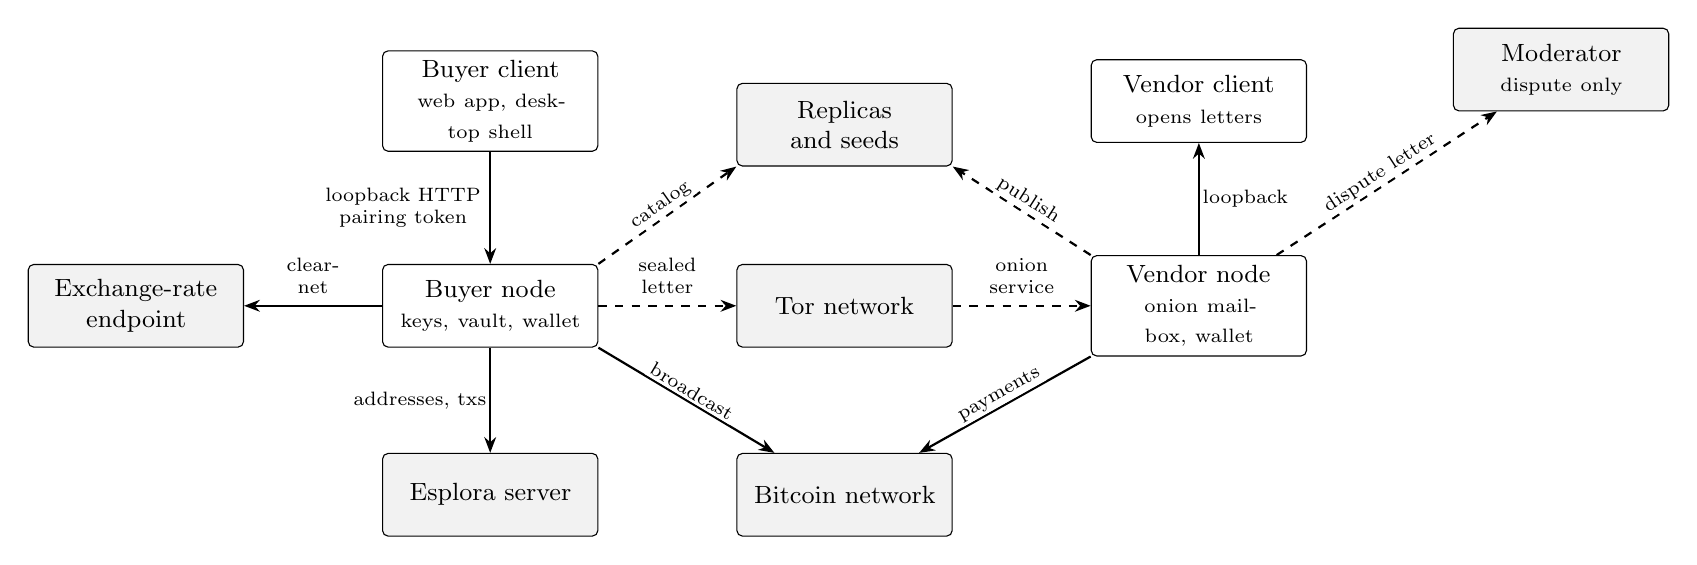
\begin{tikzpicture}[
  font=\small,
  box/.style={draw, rounded corners=2pt, align=center, minimum height=1.05cm, text width=2.5cm, fill=white},
  ext/.style={box, fill=black!5},
  impl/.style={-{Stealth[length=2mm]}, thick},
  spec/.style={-{Stealth[length=2mm]}, thick, dashed},
  lbl/.style={font=\scriptsize, align=center, fill=white, inner sep=1pt}
]
\node[box] (client) at (0,0) {Buyer client\\\scriptsize web app, desktop shell};
\node[box] (bnode) at (0,-2.6) {Buyer node\\\scriptsize keys, vault, wallet};
\node[box] (vnode) at (9.0,-2.6) {Vendor node\\\scriptsize onion mailbox, wallet};
\node[box] (vapp) at (9.0,0) {Vendor client\\\scriptsize opens letters};
\node[ext] (tor) at (4.5,-2.6) {Tor network};
\node[ext] (rep) at (4.5,-0.3) {Replicas and seeds};
\node[ext] (mod) at (13.6,0.4) {Moderator\\\scriptsize dispute only};
\node[ext] (esplora) at (0,-5.0) {Esplora server};
\node[ext] (chain) at (4.5,-5.0) {Bitcoin network};
\node[ext] (rates) at (-4.5,-2.6) {Exchange-rate\\endpoint};

\draw[impl] (client) -- node[lbl, left, xshift=-2pt]{loopback HTTP\\pairing token} (bnode);
\draw[spec] (bnode) -- node[lbl, above=3pt]{sealed\\letter} (tor);
\draw[spec] (tor) -- node[lbl, above=3pt]{onion\\service} (vnode);
\draw[impl] (vnode) -- node[lbl, right]{loopback} (vapp);
\draw[spec] (bnode.north east) -- node[lbl, sloped, above]{catalog} (rep.south west);
\draw[spec] (vnode.north west) -- node[lbl, sloped, above]{publish} (rep.south east);
\draw[impl] (bnode) -- node[lbl, left]{addresses, txs} (esplora);
\draw[impl] (bnode.south east) -- node[lbl, sloped, above]{broadcast} (chain);
\draw[impl] (vnode.south west) -- node[lbl, sloped, above]{payments} (chain);
\draw[spec] (vnode) -- node[lbl, sloped, above]{dispute letter} (mod);
\draw[impl] (bnode) -- node[lbl, above=3pt]{clear-\\net} (rates);
\end{tikzpicture}}
\caption{Components and data paths. Solid arrows exist in code on main or an open pull request; dashed arrows are specified but not implemented. In today's demonstration the buyer node and vendor node are the same process, and the sealed letter is written to that process's own mailbox directory. The phone-to-node pairing is not drawn; the client currently reaches only a node on the same machine.}
\label{fig:architecture}
\end{figure}


Figure~\ref{fig:architecture} shows the components. A user runs a client and a node. The node holds the keys, the wallet, the encrypted vault, the verified catalog, and the escrow state; it watches the chain and talks to other nodes. The client renders the catalog, the cart, and the order screens, and holds no keys.

\subsection{The client-node boundary}

A node listens only on a loopback address and refuses requests whose TCP peer is not a loopback address. On first start it creates a 256-bit random pairing token, stored in a file readable only by its owner. Requests that place orders, read or write the address book, or read the buyer's order list must carry the token. Cross-origin responses name only the client's origins, so a web page from another origin in the user's browser cannot read the token or call the node with it. A phone that pairs with a node on another machine needs an authenticated, encrypted channel to it in addition to the token; we leave that pairing transport to future work (\S\ref{sec:future}).

This boundary protects against remote callers and against other web origins in the user's browser. It does not protect against another process running as the same user on the same machine, which can read the token file; we treat that as a compromised device (A6).

Nodes leave escrow letters for each other in a drop that takes no pairing token, since the sender is another node, not the owner's client. The drop only stores the bytes. A letter has effect only if it opens under one of the node's keys and parses as an escrow message for an escrow the node is in, and every message is then checked against the signed terms (\S\ref{sec:escrow}).

The node refuses any client request that names a destination: a field such as \code{peer}, \code{onion}, \code{seed}, \code{replica}, or \code{url}, or any string value containing \code{://} or \code{.onion}. A client therefore cannot direct the node to dial an address of the client's choosing. The vendor is always the store that signed the listing the node already holds, reached at the mailbox that store published.

\subsection{Deployment}

A vendor runs a node that stays awake (a desktop computer or an Android device), publishes the catalog, runs an onion service that accepts sealed letters, and watches the chain. A buyer uses the same software; a buyer on an iPhone pairs the installed web app with their own desktop or Android node. All peer-to-peer traffic, including catalog fetches, publishing, label sets, letter delivery, and escrow messages, runs over Tor between nodes. A moderator is a node like any other, with a published record and an onion mailbox; it needs to be online only to answer disputes.

\section{Catalog and Replication}
\label{sec:catalog}

\subsection{Records}

A \emph{store record} \IT{} contains a display name, a region, two direct-payment strings (a BOLT 12 offer and a BIP 352 code), and the store's 32-byte x-only public key $S$, which is the store identifier. A \emph{listing} \IT{} contains $S$, a title, a category, a price in satoshis, a ship-from region, a description, a seller display name, a stock count, the date it was signed, whether it accepts a moderator, a kind (physical or digital), an optional shared product key, flat shipping in satoshis, and the subtotal above which shipping is waived. Neither record has a field for a legal name, an email address, a phone number, or a street address. The free-text fields are not checked for such content; rejecting it at encoding time is specified but not implemented \SP.

\subsection{Canonical encoding}

Each record body is a fixed sequence of fields \IT: a four-byte magic (\code{OBST} for stores, \code{OBLS} for listings), a one-byte version, then fields in a fixed order. Integers are little-endian of fixed width. Strings are a two-byte little-endian length followed by UTF-8 bytes; blobs are a four-byte length, capped at 8~MiB. The decoder rejects a wrong magic, a wrong version, invalid UTF-8, truncation, and trailing bytes. Because every variable-length field is length-prefixed and the field order is fixed, distinct records have distinct encodings, and a decoded record re-encodes to the same bytes (a property the tests check).

\subsection{Signatures and addresses}

The signature is a BIP 340 Schnorr signature~\citep{bip340} over a tagged hash of the body:
\[
  \sigma = \mathsf{Sign}_{s}\bigl(\Hash_{\mathrm{tag}}(\mathit{body})\bigr),\quad \Hash_{\mathrm{tag}}(m)=\mathrm{SHA256}\bigl(\mathrm{SHA256}(\mathrm{tag})\,\|\,\mathrm{SHA256}(\mathrm{tag})\,\|\,m\bigr),
\]
with tags \code{ob/store/v1} and \code{ob/listing/v1}, so a signature over one record type is not valid for another. Signing uses BIP 340's deterministic nonce derivation without auxiliary randomness. The signature is appended to the body. A listing can only be signed by the secret key of the store it names: the signing function refuses otherwise, and verification checks the signature against the $S$ inside the listing body.

A listing's address is $\mathrm{SHA256}(\mathit{body})$, computed over the body without the signature \IT. An order commits to this address, so a vendor who later edits a listing (for example, raising the price) produces a new address and cannot claim that the buyer agreed to the new terms. The node refuses an order for an address that is not in its verified catalog.

\subsection{What the signature does not give}

A valid signature proves that the store key holder signed those bytes at some time. It does not prove that the listing is current or that a set of listings is complete. A replica can serve an older, validly signed version of a listing (an old price or stock count), and it can omit listings entirely, without either being detectable by signature checks alone. Addressing a listing by content hash makes an order unambiguous about which version it bought, but does not tell a buyer whether a newer version exists. A per-store sequence number or a signed index of current listings would address freshness and completeness; neither is designed in detail \FW.

\subsection{Replication}

The intended design \SP{} has every node store the signed headers of the catalog it has seen, so that a store remains browsable while its publisher is offline, and requires images and files to be held by at least one replica before a listing counts as published. Because records are self-authenticating, a replica needs no trust for integrity: a client or node that receives a record from anyone checks the signature and the content hash. Replicas are trusted only for availability and see who fetches what (\S\ref{sec:privacy}).

An open catalog invites spam. The design calls for each published header to carry a cost that receiving nodes check, such as a small bitcoin fee \SP; no fee mechanism is designed in detail, and none is implemented. Until one exists, replication would be limited to stores a node has chosen to follow or has received through a pasted link.

On main, the catalog is a fixture of one store and 38 listings across three sellers, signed at startup with fixture keys and verified before it is served \ID. In the fixture, the three sellers are display names on listings under a single store key; the protocol itself assigns one store key per vendor.

\section{Identity and Keys}
\label{sec:identity}

\subsection{Key roles}

The design gives each user one backup phrase and derives a separate key for each role, so that a key used to sign the public catalog is never the key that spends coins. PR~\#2 implements this \IT{} with a 12-word BIP 39 phrase~\citep{bip39} and BIP 32 derivation~\citep{bip32}:

\begin{center}\small
\begin{tabular}{@{}ll@{}}
\toprule
\textbf{Role} & \textbf{Derivation path} \\
\midrule
Spend wallet (BIP 86 Taproot~\citep{bip86}) & \code{m/86'/c'/0'/\{0,1\}/*} \\
Store signing key & \code{m/1984'/c'/0'/0'} \\
Escrow key $i$ & \code{m/1984'/c'/1'/i'} \\
BIP 352 scan key & \code{m/352'/c'/0'/1'/0} \\
BIP 352 spend key & \code{m/352'/c'/0'/0'/0} \\
\bottomrule
\end{tabular}
\end{center}

The coin type $c$ is 0 on mainnet and 1 on testnet4, and each network has its own data directory, so a phrase used on both networks never yields the same key on both. A test checks that all role keys are pairwise distinct across both networks. Escrow keys are indexed, and the index is advanced and persisted before a key is used, so each escrow gets a new key.

On main, every key is a fixture: a scalar computed by hashing a fixed label \ID. The demonstration node holds the store key, the vendor spend and scan keys, a buyer key, and the moderator's secret key in one process. Those fixtures exist so the demonstration can run end to end on one machine; they are not a security configuration.

\subsection{The mailbox key}

Orders are sealed to an X25519 public key belonging to the vendor (\S\ref{sec:orders}). That key must be bound to the store, so that a buyer who verified a listing also knows which key to seal to. The intended binding is a field in the signed store record \SP. Today the store record has no such field: the node looks up the vendor's mailbox key in a fixture table keyed by seller display name \ID. For one fixture seller, the mailbox key is the same 32-byte string as the store's secp256k1 signing key, interpreted as an X25519 scalar. Reusing one secret across two groups and two protocols has no known attack in this specific combination, but it is poor hygiene; the mailbox key should be derived on its own path \SP.

\subsection{Encryption at rest}

The node stores the buyer's address book and the buyer's own order records encrypted with ChaCha20-Poly1305 under a random 256-bit key and a random 96-bit nonce per write \IT. PR~\#2 stores the BIP 39 phrase and the wallet state the same way \IT. The key is in a file named \code{vault.key}, mode \code{0600}, in the same data directory.

This protects against the encrypted files being copied or synced on their own, for example by a backup tool that skips key files, and keeps addresses out of logs and the catalog. It does not protect against anyone who can read the data directory, since the key sits beside the ciphertext. It is not a defense against a compromised device (A6). Wrapping the key with an operating-system keystore or a passphrase is not implemented.

The buyer's order record keeps the label of the address used (for example, ``Home''), not the street.

\section{Order Sealing and Transport}
\label{sec:orders}

\begin{figure}[t]
\centering
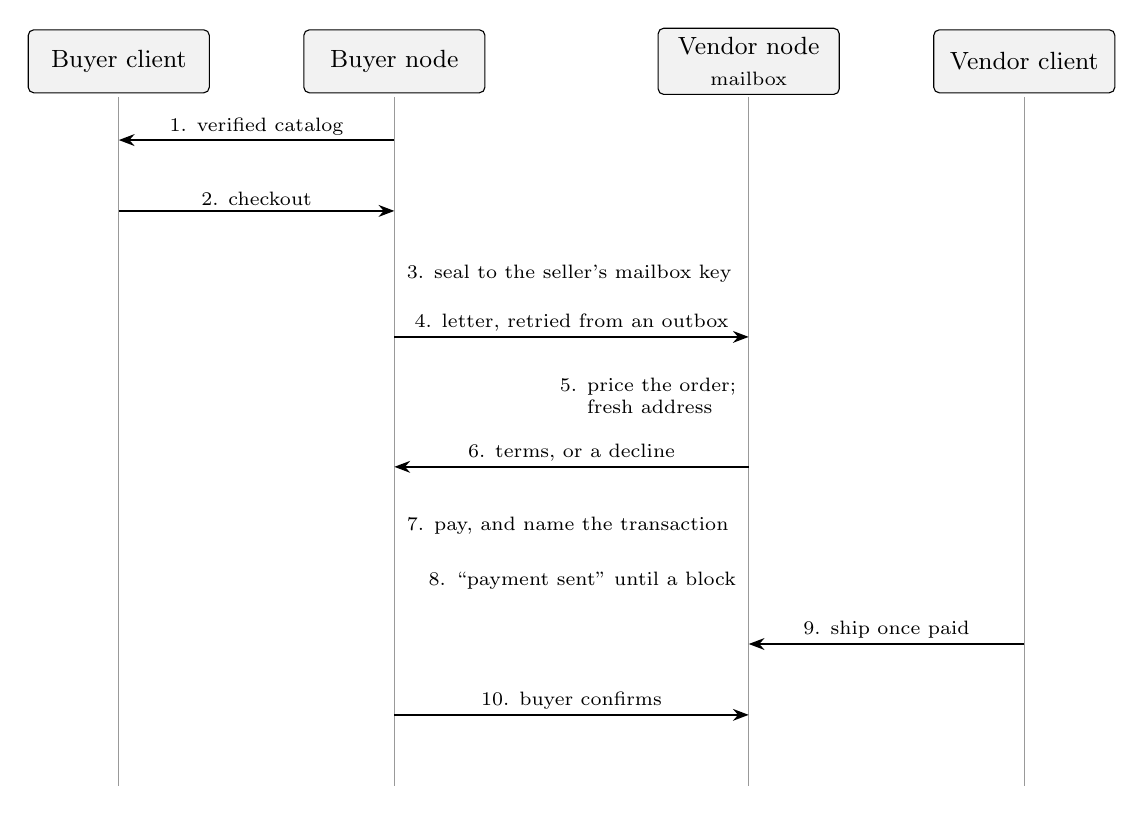
\begin{tikzpicture}[
  font=\small,
  head/.style={draw, rounded corners=2pt, fill=black!5, align=center, minimum width=2.3cm, minimum height=0.8cm},
  msg/.style={-{Stealth[length=2mm]}, thick},
  note/.style={font=\scriptsize, align=left, fill=white, inner sep=1.5pt},
]
\def\xc{0} \def\xb{3.5} \def\xv{8.0} \def\xa{11.5}
\node[head] (hc) at (\xc,0) {Buyer client};
\node[head] (hb) at (\xb,0) {Buyer node};
\node[head] (hv) at (\xv,0) {Vendor node\\\scriptsize mailbox};
\node[head] (ha) at (\xa,0) {Vendor client};
\foreach \x in {\xc,\xb,\xv,\xa} { \draw[black!40] (\x,-0.45) -- (\x,-9.2); }

\draw[msg] (\xb,-1.0) -- node[note, above]{1. verified catalog} (\xc,-1.0);
\draw[msg] (\xc,-1.9) -- node[note, above]{2. checkout} (\xb,-1.9);
\node[note, right] at (\xb+0.1,-2.7) {3. seal to the seller's mailbox key};
\draw[msg] (\xb,-3.5) -- node[note, above]{4. letter, retried from an outbox} (\xv,-3.5);
\node[note, left] at (\xv-0.1,-4.25) {5. price the order;\\\phantom{5. }fresh address};
\draw[msg] (\xv,-5.15) -- node[note, above]{6. terms, or a decline} (\xb,-5.15);
\node[note, right] at (\xb+0.1,-5.9) {7. pay, and name the transaction};
\node[note, left] at (\xv-0.1,-6.6) {8. ``payment sent'' until a block};
\draw[msg] (\xa,-7.4) -- node[note, above]{9. ship once paid} (\xv,-7.4);
\draw[msg] (\xb,-8.3) -- node[note, above]{10. buyer confirms} (\xv,-8.3);
\end{tikzpicture}
\caption{A sale between two nodes (\S\ref{sec:sale}). Steps 4, 6, and 10 are sealed letters to the other node's loopback mail endpoint. The seller shows step 8 because compact filters cannot see the mempool. A multi-seller checkout repeats the exchange once per seller.}
\label{fig:orderflow}
\end{figure}


An order is a private letter to one vendor, not a catalog record and not an event on a public relay. Figure~\ref{fig:orderflow} shows the flow.

\subsection{Order contents}

The order plaintext (magic \code{OBOD}, version 1) contains: the address of the first listing; its quantity; an options map of up to 16 string pairs, which carries the settlement type, the shipping charge, a delivery note for digital goods, and the address and quantity of any further listings from the same seller; the ship-to text (at most 1024 bytes) for physical goods; the payment rail; and a fresh X25519 public key $R$ that the vendor uses to reply. The order carries no long-term buyer identity key and no buyer signature. The vendor learns who the buyer is only from what the buyer writes into the letter (for a physical good, the ship-to) and from the payment.

\subsection{Sealing}

The node seals the plaintext with HPKE~\citep{rfc9180} in base mode with the suite DHKEM(X25519, HKDF-SHA256)~\citep{rfc7748,rfc5869}, HKDF-SHA256, and ChaCha20-Poly1305~\citep{rfc8439}. The recipient key is the vendor's mailbox key $P_V$; the HPKE \code{info} string is \code{openbazaar-tormail-order-v1}; the associated data is empty. The sealed letter is
\[
  \code{OBSL} \,\|\, \mathtt{0x01} \,\|\, \mathit{enc} \,\|\, \mathrm{len}_{32}(\mathit{ct}) \,\|\, \mathit{ct},
\]
where $\mathit{enc}$ is HPKE's 32-byte encapsulated ephemeral key. Letters larger than 64~KiB are rejected. A vendor reply is sealed the same way to the buyer's per-order key $R$ with \code{info} \code{openbazaar-tormail-reply-v1} and a size limit of 8~KiB. Because $R$ is generated per order and travels inside the ciphertext, no relay or mailbox needs to remember which buyer wrote to which vendor in order to route a reply.

Base mode means letters are not authenticated to a sender: anyone who knows $P_V$ can produce a letter that the vendor will decrypt. This is deliberate, since a buyer should not need a long-term identity to order, but it means the vendor must treat an order as an offer that becomes real when paid. It also means that a vendor's mailbox can be filled with junk letters; the mailbox caps letter size but does not rate-limit.

Letters are not padded. The ciphertext is exactly 16 bytes longer than the plaintext, so an observer who sees a letter at rest or in transit learns its length, which correlates with the length of the ship-to and the number of lines. Over Tor, a letter of a few hundred bytes fits in a small number of fixed-size cells, which hides the exact length from relays but not the approximate size. Padding to fixed size buckets would hide it (\S\ref{sec:future}).

\subsection{Multi-seller checkout}

A checkout may contain packages from several sellers. The node validates every package (each listing exists in the verified catalog, each package is one seller and each seller one package, moderated packages only contain listings that accept the moderator) before sealing anything, then seals one letter per seller to that seller's key. A seller learns only the lines in its own package. Each package gets its own payment instructions and its own payment (\S\ref{sec:payments}).

\subsection{The mailbox}

The vendor's node accepts letters into a mailbox directory without loading any secret: a letter is written to a temporary file and renamed to a random 128-bit identifier, so the identifier is not derived from the sender. Letters are opened later with the mailbox secret. A node that is compromised while the vendor is away therefore holds ciphertext, not orders, unless the mailbox secret is also stored on it.

\subsection{Transport}

Letters travel over Tor~\citep{dingledine2004tor}. The vendor's node runs a v3 onion service~\citep{torrendv3} whose address is published with its store record. The buyer's node dials it on a fixed virtual port and writes one framed letter (\code{OBML}, version 1); the listener accepts one stream per rendezvous, rejects streams for any other port, and writes the letter into the mailbox. If the vendor's node is unreachable, the buyer's node keeps the letter in an outbox and retries until a deadline, after which the buyer is told the order was not delivered. No third-party relay stores letters: a vendor whose node is never awake is a closed shop. Escrow letters (\S\ref{sec:escrow}) and dispute letters use the same transport to the counterparty's or moderator's onion mailbox.

Using an onion service for the vendor's mailbox means the vendor's IP address is not revealed to buyers, and the buyer's node connects through a Tor circuit, so the vendor does not learn the buyer's IP address. Tor does not protect against an adversary who observes both ends of a circuit~\citep{dingledine2004tor,johnson2013users}; \S\ref{sec:privacy} discusses this. Carrying letters over a mix network such as Nym~\citep{diaz2021nym,piotrowska2017loopix} to resist timing correlation is future work (\S\ref{sec:future}).

\section{Payments}
\label{sec:payments}

All payments are in bitcoin. There is no swap service, mixer, ecash mint, or second asset in the design or the code. Direct payment goes from the buyer to the vendor with no intermediary; moderated payment goes through the escrow of \S\ref{sec:escrow}.

\subsection{One payment per seller}

A multi-seller checkout produces one order per seller, and each order is paid by its own transaction \IT{} (PR~\#2). The pay-from-node path builds a transaction with exactly one recipient output and, if needed, one change output back to the buyer's own wallet. Two sellers are never paid in one transaction, because a transaction with outputs to two vendors would tell anyone watching the chain that the same person bought from both.

Separate transactions are necessary for unlinkability, not sufficient. If the wallet funds the second payment with the change from the first, the common-input-ownership and change heuristics~\citep{meiklejohn2013fistful} link the two payments. At \paycommit{} coin selection skips unconfirmed coins received from others but deliberately keeps the wallet's own unconfirmed change spendable, so paying two sellers in quick succession can chain the second payment onto the first payment's change. The wallet does not currently avoid this; choosing inputs so that one checkout's payments do not share ancestry is future work \FW.

\subsection{On-chain direct payment}

In PR~\#2, each direct order receives a fresh receive address from the vendor's BDK descriptor wallet (BIP 86 Taproot) and a BIP 21~\citep{bip21} URI for the exact amount \IT. The node's chain watcher queries an Esplora server for transactions paying each watched address and marks an order as payment seen and then paid once the required confirmations (one on testnet4, three by default on mainnet) are reached. The node can also pay an order from its own wallet. The default network is testnet4~\citep{bip94}. Mainnet is selected only by the exact flag \code{--network mainnet}, and a mainnet payment from the node additionally requires \code{"confirm": true} in the request.

Because the demonstration node holds both the buyer wallet and the vendor wallets, a single node can both pay and observe an order \ID. In a deployment the buyer and vendor nodes are different machines, and each watches only its own addresses.

\paragraph{The Esplora server.} Every chain query names a specific address to the Esplora server~\citep{esplora}. The defaults are \code{mempool.space} on mainnet and, on testnet4, \code{mempool.space} with \code{blockstream.info} as an ordered fallback; the node checks that each server's genesis block matches its network before using it. Whichever server answers learns the full set of addresses the node watches, their timing, and the IP address of the node, which together link a user's orders to each other and to a network location; once the node falls back, the second operator learns the same. On mainnet the node prints a warning when the server is public. Routing chain queries over Tor \SP{} would hide the IP address but not the address set; running one's own Esplora or Bitcoin Core node, or using compact block filters, would hide both. None of these is implemented.

\subsection{Lightning: BOLT 12}

A store record carries a BOLT 12 offer~\citep{bolt12}, and direct checkout returns an offer for the order's exact amount \status{encoding only}. The offer is a valid \code{lno1} string built with LDK's offer builder, signed with the store's signing public key, and carrying no blinded path. No Lightning node in the system answers invoice requests for it, so it cannot be paid today.

Two privacy points apply once it can. An offer without a blinded path names the issuer's node key, so the offer links the store to a Lightning node. Using the store signing key as the offer's issuer key, as the current code does, also links the catalog identity to that Lightning identity; a separate key is the intended design \SP. On a payment, every routing hop sees the amount it forwards and its neighbors; the recipient's position is hidden from the payer only to the extent that a blinded path of more than one hop is used~\citep{kappos2021lightning}.

\subsection{Silent payments: BIP 352}

The store record also carries a BIP 352 silent-payment code~\citep{bip352} \status{encoding only}. A silent-payment code lets a payer derive a fresh output for each payment from a static public code, so a single published code does not lead to address reuse. The code is constructed from the scan and spend public keys and parsed with checksum validation. The node does not scan the chain for payments to the code. A buyer who pays the code today creates an output the vendor's node will not detect until scanning exists; the funds are recoverable with the scan and spend keys but the order would not be marked paid. The intended design keeps the scan key, which is watch-only, on the vendor's node so that scanning does not hand the key to a public indexer \SP.

\subsection{Payjoin: BIP 77}

Payjoin v2~\citep{bip77} lets a receiver add an input to the buyer's transaction through an asynchronous directory reached over Oblivious HTTP~\citep{rfc9458}, which breaks the assumption that all inputs belong to the payer. The \code{pay} crate wraps the \code{payjoin} library's v2 sender and receiver sessions and the step where the vendor contributes an input \status{library only}. No checkout starts a Payjoin session, and the payment terms carry no \code{pj=} endpoint. When Payjoin is used, the vendor learns which coins the buyer spent, and the buyer learns one of the vendor's coins.

\subsection{What the chain shows}

For an on-chain direct payment, a chain observer sees an ordinary transaction with one or two outputs. The amount is the listing price times quantity plus shipping. Prices are public, so an amount that matches a distinctive price can identify the listing that was bought, even though nothing else in the transaction refers to OpenBazaar. Round prices reduce this and do not remove it. For escrow, see \S\ref{sec:escrow-privacy}.

\section{Scriptless Escrow}
\label{sec:escrow}

A moderated purchase protects the buyer against non-delivery and the vendor against a buyer who will not release payment, with a moderator to decide disputes. The original OpenBazaar used a 2-of-3 multisignature script for this. The redesign keeps the economic model (a moderator together with one party can decide the outcome) and changes three things: the moderator holds no key over the funds; every outcome looks like an ordinary single-key Taproot spend; and the moderator can choose only between two payouts that buyer and vendor both signed before funding.

This section first states what is merged and what the open escrow pull request changes, then specifies the two-party protocol.

\subsection{Status of the escrow code}
\label{sec:escrow-status}

\paragraph{Merged (main).} The escrow crate on main computes a MuSig2 key-path funding output, presigns a locktime refund, and builds adaptor signatures for both dispute outcomes \ID. It does all of this in one function, \code{fund}, that takes both the buyer's and the vendor's secret keys. A review of the merged code found that, in addition: the node calls it with fixture keys; the funding outpoint is synthetic; the presigned refund is not kept by the node; there is no presigned vendor default, so a buyer who stops responding cannot be overridden before the refund height; the encrypted moderator halves carry no proof that they decrypt to the right value; there is no moderator fee; network fees are zero; and the funding address is the same for every order between the same buyer and vendor keys. The merged escrow is a demonstration of the transaction shapes, not a protocol between two parties.

\paragraph{PR~\#2.} The payments branch keeps the single-process ceremony but restricts it to testnet4 (mainnet refuses escrow), derives a new escrow key per order for each side, adds a 500-satoshi spend fee, and enforces the order ``sign the funding transaction, run the ceremony for that exact outpoint, check and store the refund, then broadcast'' \ID. Its responses mark escrow as an unsafe demonstration.

\paragraph{PR~\#3.} The two-party protocol below is implemented \IT{} in the escrow crate on branch \code{escrow-two-party} (we ran its 26 unit tests and 3 doctests). Each party's state machine holds only that party's secret key, and the parties exchange three serializable messages. The node does not call this protocol yet, no transport carries its messages, and the old single-process function remains behind a deprecated feature so the node demonstration still builds. Everything in \S\ref{sec:escrow-notation}--\S\ref{sec:escrow-privacy} describes PR~\#3; we note where its behavior depends on a caller obligation that no code yet fulfills.

\subsection{Notation}
\label{sec:escrow-notation}

$G$ generates the secp256k1 group of prime order $n$. Lowercase letters are scalars and uppercase letters are points. $\Hash_{\mathrm{tag}}$ is a BIP 340 tagged hash.

\begin{itemize}
  \item Long-term keys: buyer $(\bar b,\bar B)$, vendor $(\bar v,\bar V)$. Moderator $(k,K)$.
  \item Order secret $s$: 32 bytes known only to buyer and vendor. Per-order keys $b=\bar b+\Hash_{\mathrm{ord}}(\bar B,s)$ and $B=bG$, and likewise $v$, $V$.
  \item Aggregate key: $P=\mathsf{KeyAgg}(B,V)$ under BIP 327~\citep{bip327} with the two keys sorted; output key $Q=P+\Hash_{\mathrm{TapTweak}}(P)\,G$, the BIP 341~\citep{bip341} tweak with no script tree. The funding output is P2TR with output key $Q$ and value $F$.
  \item Terms $\tau=(B,V,K,F,f,\varphi,h_D,h_C,h_R,S_B,S_V,S_M)$: network fee $f$, moderator fee $\varphi$, dispute deadline $h_D$, vendor claim height $h_C$, refund height $h_R$, and payout scripts for buyer, vendor, and moderator. Both parties sign $\tau$; the signed terms are $\tau^\ast$.
  \item Outpoint $o$ of the funding output.
  \item For a dispute branch favoring party $X\in\{B,V\}$, with $\bar X$ the other party: the \emph{party half} $t_X$, $T_X=t_XG$, derived by $X$ from its per-order secret key and the branch; the \emph{moderator half} $u_X$, $U_X=u_XG$, sampled by $\bar X$; the adaptor point $Y_X=T_X+U_X$.
  \item $\mathsf{VEnc}_K(u;\mathit{ctx})$: verifiable encryption of $u$ to $K$, bound to context $\mathit{ctx}$ (\S\ref{sec:vencrypt}). $\pi^{\mathrm{pok}}(t)$: Schnorr proof of knowledge of $t$.
\end{itemize}

\begin{figure}[t]
\centering
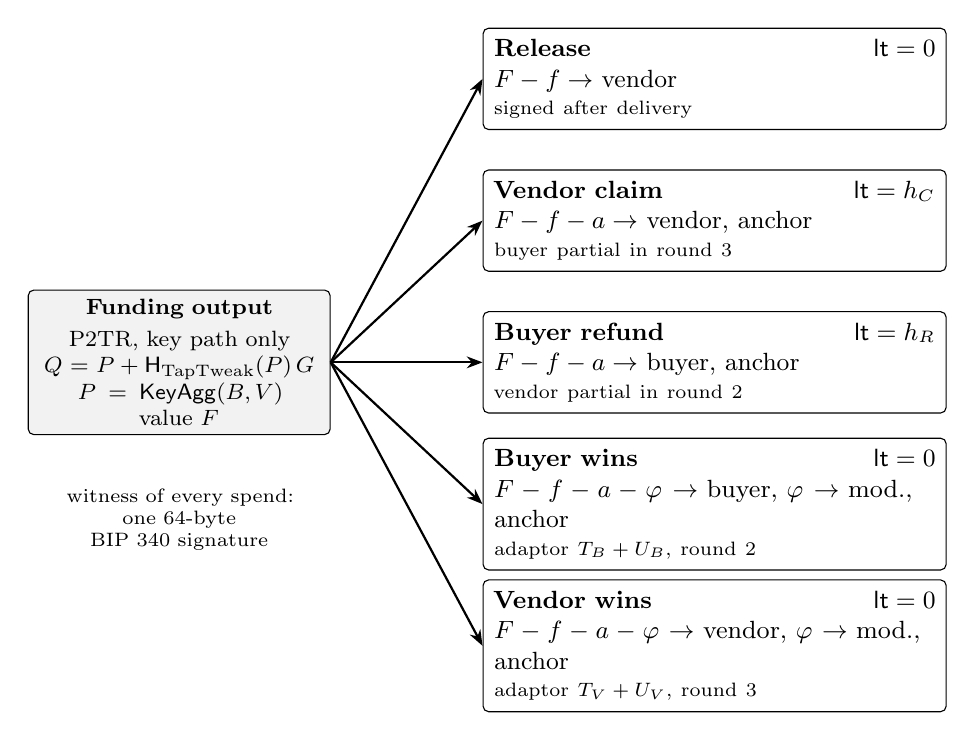
\begin{tikzpicture}[
  font=\small,
  txb/.style={draw, rounded corners=2pt, align=left, text width=5.6cm, minimum height=1.0cm, fill=white, inner sep=4pt},
  fund/.style={draw, rounded corners=2pt, align=center, text width=3.6cm, minimum height=1.6cm, fill=black!5, font=\footnotesize},
  arr/.style={-{Stealth[length=2mm]}, thick},
]
\node[fund] (f) at (0,0) {\textbf{Funding output}\\[2pt] P2TR, key path only\\ $Q = P + \Hash_{\mathrm{TapTweak}}(P)\,G$\\ $P=\mathsf{KeyAgg}(B,V)$\\ value $F$};
\node[txb] (rel) at (6.8,3.6)  {\textbf{Release} \hfill $\mathsf{lt}=0$\\ $F-f \to$ vendor\\[-1pt]\scriptsize signed after delivery};
\node[txb] (clm) at (6.8,1.8) {\textbf{Vendor claim} \hfill $\mathsf{lt}=h_C$\\ $F-f-a \to$ vendor, anchor\\[-1pt]\scriptsize buyer partial in round 3};
\node[txb] (ref) at (6.8,0)    {\textbf{Buyer refund} \hfill $\mathsf{lt}=h_R$\\ $F-f-a \to$ buyer, anchor\\[-1pt]\scriptsize vendor partial in round 2};
\node[txb] (bw)  at (6.8,-1.8){\textbf{Buyer wins} \hfill $\mathsf{lt}=0$\\ $F-f-a-\varphi \to$ buyer, $\varphi\to$ mod., anchor\\[-1pt]\scriptsize adaptor $T_B+U_B$, round 2};
\node[txb] (vw)  at (6.8,-3.6) {\textbf{Vendor wins} \hfill $\mathsf{lt}=0$\\ $F-f-a-\varphi \to$ vendor, $\varphi\to$ mod., anchor\\[-1pt]\scriptsize adaptor $T_V+U_V$, round 3};
\foreach \t in {rel,clm,ref,bw,vw} { \draw[arr] (f.east) -- (\t.west); }
\node[font=\scriptsize, align=center, text width=3.4cm] at (0,-2.0) {witness of every spend:\\one 64-byte BIP~340 signature};
\end{tikzpicture}
\caption{Escrow transaction graph. All five spends are key-path spends of the same output under the MuSig2 aggregate of the buyer's and vendor's per-order keys; the moderator's key is not part of $Q$. Four spends are presigned before funding; the release is signed cooperatively later. $f$ is the network fee, $\varphi$ the moderator fee, and $a$ the 240-satoshi pay-to-anchor output, all fixed by the signed terms; $\mathsf{lt}$ is \code{nLockTime}.}
\label{fig:escrow-graph}
\end{figure}

\begin{figure}[t]
\centering
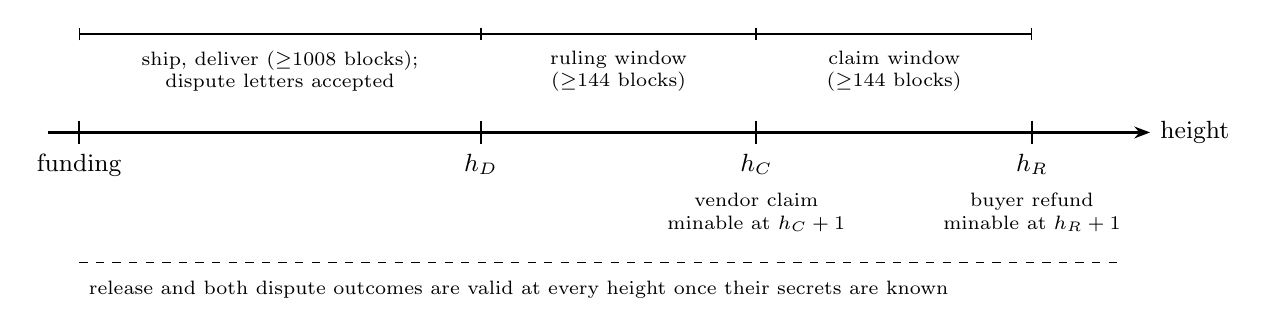
\begin{tikzpicture}[font=\small, >={Stealth[length=2mm]}]
\draw[->, thick] (0,0) -- (14,0) node[right]{height};
\foreach \x/\l in {0.4/funding, 5.5/$h_D$, 9.0/$h_C$, 12.5/$h_R$} {
  \draw[thick] (\x,0.15) -- (\x,-0.15);
  \node[below] at (\x,-0.15) {\l};
}
\draw[|-|] (0.4,1.25) -- (5.5,1.25);
\node[above, align=center, font=\scriptsize] at (2.95,0.4) {ship, deliver ($\ge$1008 blocks);\\dispute letters accepted};
\node[above, align=center, font=\scriptsize] at (7.25,0.4) {ruling window\\($\ge$144 blocks)};
\node[above, align=center, font=\scriptsize] at (10.75,0.4) {claim window\\($\ge$144 blocks)};
\draw[|-|] (5.5,1.25) -- (9.0,1.25);
\draw[|-|] (9.0,1.25) -- (12.5,1.25);
\node[below, align=center, font=\scriptsize] at (9.0,-0.65) {vendor claim\\minable at $h_C+1$};
\node[below, align=center, font=\scriptsize] at (12.5,-0.65) {buyer refund\\minable at $h_R+1$};
\draw[dashed] (0.4,-1.65) -- (13.6,-1.65);
\node[font=\scriptsize, align=left, anchor=west] at (0.4,-2.0) {release and both dispute outcomes are valid at every height once their secrets are known};
\end{tikzpicture}
\caption{Escrow timeline. The default after $h_C$ is the vendor; the refund at $h_R$ matters only if the vendor never claims. Window sizes are policy minimums checked by each party at funding against the current tip; the minimums are 1{,}008 blocks from the tip to $h_D$ and 144 blocks for each later window.}
\label{fig:escrow-timeline}
\end{figure}


\subsection{Terms and transactions}

Before any funding round, the parties agree on $\tau$ and each checks it under its own local policy: the three keys are distinct; $0<h_D<h_C<h_R$ are block heights with $h_C-h_D$ and $h_R-h_C$ at least a minimum window (144 blocks each by default); the moderator fee is at least the P2TR dust limit of 330 satoshis; every payout is at least dust; and every presigned transaction meets a minimum fee rate measured on its actual signed size \IT. The moderator key must match the key the party already trusts from the listing, so a counterparty cannot substitute a different moderator \IT.

From $\tau$ and $o$, each party derives the same five spends (Figure~\ref{fig:escrow-graph}). Each has one input spending $o$ with sequence \code{0xfffffffe} (so \code{nLockTime} is enforced) and is signed as a BIP 341 key-path spend with \code{SIGHASH\_DEFAULT}:
\begin{center}\small
\begin{tabular}{@{}llll@{}}
\toprule
\textbf{Spend} & \code{nLockTime} & \textbf{Outputs} & \textbf{When signed} \\
\midrule
$\tx{rel}$ (release) & 0 & $F-f\to S_V$ & cooperatively, after delivery \\
$\tx{clm}$ (vendor claim) & $h_C$ & $F-f\to S_V$ & presigned (buyer, round 3) \\
$\tx{ref}$ (buyer refund) & $h_R$ & $F-f\to S_B$ & presigned (vendor, round 2) \\
$\tx{B}$ (buyer wins) & 0 & $F-f-\varphi\to S_B$, $\varphi\to S_M$ & adaptor $Y_B$ (vendor, round 2) \\
$\tx{V}$ (vendor wins) & 0 & $F-f-\varphi\to S_V$, $\varphi\to S_M$ & adaptor $Y_V$ (buyer, round 3) \\
\bottomrule
\end{tabular}
\end{center}
A transaction with \code{nLockTime} $h$ can first be mined in block $h+1$.

\subsection{Funding rounds}

Let $\mathsf{N}$ denote a party's MuSig2 public nonces for the four presigned spends and $\mathsf{ps}(\cdot)$ a MuSig2 partial signature~\citep{nick2021musig2} (or partial adaptor signature, for $\tx{B}$ and $\tx{V}$).

\begin{description}[leftmargin=1.2em]
  \item[Round 0.] Both parties sign $\tau$.
  \item[Round 1, buyer $\to$ vendor.] The buyer prepares, but does not sign or broadcast, a funding transaction from native segwit inputs, so its transaction id is fixed before signing. It sends
  $\bigl(o,\ \mathsf{N}_B,\ T_B,\ \pi^{\mathrm{pok}}(t_B),\ \mathsf{VEnc}_K(u_V;\mathit{ctx}_V)\bigr)$.
  The buyer samples $u_V$ because the buyer loses branch $V$.
  \item[Round 2, vendor $\to$ buyer.] The vendor checks $\pi^{\mathrm{pok}}(t_B)$ and the encryption proof for $U_V$ (it is the favored party in branch $V$, so it must be sure the moderator can reveal $u_V$). It replies
  $\bigl(\mathsf{N}_V,\ T_V,\ \pi^{\mathrm{pok}}(t_V),\ \mathsf{VEnc}_K(u_B;\mathit{ctx}_B),\ \mathsf{ps}_V(\tx{ref}),\ \mathsf{ps}_V(\tx{B};Y_B)\bigr)$.
  \item[Round 3, buyer $\to$ vendor.] The buyer checks $\pi^{\mathrm{pok}}(t_V)$ and the encryption proof for $U_B$, adds its own partial signatures, and verifies that the completed refund is a valid signature under $Q$ for the exact outpoint and value, and that the buyer-wins pre-signature is valid for $Y_B$. Only after these checks does the buyer's state machine release the funding transaction for signing \IT. The buyer must persist the refund before funding; the crate exposes it for storage and re-verification, and storing it is the caller's obligation. The buyer sends
  $\bigl(\mathsf{ps}_B(\tx{clm}),\ \mathsf{ps}_B(\tx{V};Y_V)\bigr)$.
  The vendor completes and stores the claim and verifies the vendor-wins pre-signature.
  \item[Funding.] The buyer signs and broadcasts the funding transaction. The vendor's state machine checks that a transaction creates exactly the agreed output at $o$; shipping only after that transaction confirms is the caller's obligation.
\end{description}

Each state is consumed by value when it advances, and secret nonces live only inside those states, so a nonce cannot be reused for two messages by accident. The release uses fresh nonces generated later.

\paragraph{Why each piece is there.}
\begin{itemize}
  \item \emph{Refund before funding.} The buyer never signs the funding transaction until it holds a refund that verifies against the aggregate key. A vendor who aborts after round 1 costs the buyer nothing.
  \item \emph{Claim before refund.} The buyer presigns a claim at $h_C<h_R$, so a buyer who received the goods and stops responding loses at $h_C+1$.
  \item \emph{Proof of knowledge on $T_X$.} Without it, $X$ could choose $T_X=T'-U_X$ for a $T'$ whose discrete log it knows, making $Y_X=T'$ and letting $X$ complete its own winning branch without the moderator.
  \item \emph{Verifiable encryption of $u_X$.} Without it, the losing party $\bar X$ could encrypt a value that does not match $U_X$, and the moderator would be unable to rule for $X$.
  \item \emph{Per-order keys.} Tweaking each long-term key with the order secret gives a different $Q$ for every order between the same two parties, so funding outputs between repeat trading partners are not linkable by address \IT. The protocol assumes $s$ is shared only by buyer and vendor; carrying it inside the sealed order letter is the intended channel \SP.
\end{itemize}

\subsection{Release}

When the buyer is satisfied, the vendor sends a fresh public nonce for $\tx{rel}$, and the buyer returns its nonce and partial signature. The vendor aggregates them into a 64-byte signature and broadcasts \IT. The moderator is not involved.

\subsection{Disputes}

Before $h_D$, either party $X$ can ask the moderator to rule for it by sending a \emph{dispute letter} \IT:
\[
  L_X = \bigl(\tau^\ast,\ o,\ F,\ \mathit{script}(Q),\ Q,\ X,\ \tx{X}\ \text{(unsigned)},\ T_X,\ \mathsf{VEnc}_K(u_X),\ \hat\sigma_X,\ \mathit{memo}\bigr)\ \text{signed by } X.
\]
Here $\hat\sigma_X$ is the aggregated adaptor pre-signature on $\tx{X}$ for $Y_X$. The letter is self-verifying: the moderator checks the signed terms against its own key, recomputes $P$, $Q$, the funding script, and $\tx{X}$ from the terms and outpoint, checks that $\hat\sigma_X$ is a valid pre-signature on $\tx{X}$ for $T_X+U_X$, checks the encryption proof, and checks $X$'s signature over the letter. It refuses a letter that arrives after $h_D$. Only then does it decrypt $u_X$.

If it rules for $X$, the moderator returns a \emph{ruling} $(o, X, Y_X, u_X)$ signed with $k$. $X$ computes $t_X+u_X$, completes $\hat\sigma_X$ into a valid BIP 340 signature, and broadcasts $\tx{X}$, which pays $X$ and the moderator's fee.

A ruling for $X$ is useless to $\bar X$, because $\bar X$ does not know $t_X$. A moderator that signs rulings for both branches of the same outpoint produces two signed rulings that together are transferable proof of equivocation \IT. Equivocation is detectable, not preventable: both dispute outcomes are valid from height 0, so if both parties receive a ruling, the first to confirm wins.

\subsection{Timeline}

Figure~\ref{fig:escrow-timeline} shows the heights.
\begin{itemize}
  \item From funding until $h_D$, the vendor ships, the buyer receives, and either party may send a dispute letter.
  \item Between $h_D$ and $h_C$, the moderator rules and the winner must confirm its outcome. A buyer who wins must confirm $\tx{B}$ before $h_C+1$, when $\tx{clm}$ also becomes valid.
  \item At $h_C+1$, the vendor can claim. A vendor who never claims leaves the funds in the output until $h_R+1$, when the buyer's refund becomes valid. If the vendor's claim is not confirmed by then, both are valid and the first to confirm wins.
\end{itemize}

The default outcome is therefore the vendor's. We considered and rejected a design in which the default flips to the buyer until the vendor posts a shipping attestation: without a trusted third party that observes shipping, such an attestation is not a cryptographic event, and a buyer who wants to cheat would decline to countersign it. The consequence is that a buyer who did not receive the goods must open a dispute before $h_D$.

\subsection{Moderator fee}
The moderator fee is an output of each dispute outcome and of nothing else, and it is fixed in the signed terms \IT. It is collected only when the winner broadcasts the dispute outcome. A vendor who wins a ruling close to $h_C$ can skip the fee by waiting for the fee-free claim; a buyer who wins cannot. That skews moderator income toward rulings for the buyer. A fee bond posted at funding would remove the skew and is not implemented \FW.

\subsection{Verifiable encryption of the moderator half}
\label{sec:vencrypt}

The moderator half $u$ with $U=uG$ is encrypted bit by bit with exponential ElGamal under $K$ \IT. For each bit $\beta_i$ of $u$ ($i=0,\dots,255$), the encryptor picks $r_i$ and publishes $(A_i,C_i)=(r_iG,\ r_iK+\beta_iG)$ with a Cramer--Damg{\aa}rd--Schoenmakers OR proof~\citep{cramer1994} of two Chaum--Pedersen statements~\citep{chaum1992} showing that $\beta_i\in\{0,1\}$. A Chaum--Pedersen proof then shows
\[
  \log_G\Bigl(\textstyle\sum_i 2^iA_i\Bigr)=\log_K\Bigl(\textstyle\sum_i 2^iC_i-U\Bigr),
\]
which holds exactly when $\sum_i 2^i\beta_i\equiv u \pmod n$. Anyone with $K$ and $U$ can check the ciphertext; only the holder of $k$ can decrypt, since $C_i-kA_i$ is either the identity or $G$. All challenges are tagged hashes over length-prefixed inputs and a 32-byte context that binds the proof to one escrow branch. This is the bitwise approach to verifiable encryption of a discrete logarithm~\citep{stadler1996pvss,camenisch2003}. Its cost is size: one encrypted share is 49{,}761 bytes (\S\ref{sec:evaluation}).

\subsection{What the chain shows}
\label{sec:escrow-privacy}

Every spend is a single-input Taproot key-path spend with one 64-byte signature. No script, no moderator key, and no multisignature structure appears on chain in any outcome, including a dispute \IT. This is the main privacy improvement over the original 2-of-3 design. What remains visible:
\begin{itemize}
  \item The funding amount $F$ (price plus shipping plus fees), which can point to a listing with a distinctive price.
  \item Dispute outcomes have two outputs, one of which is the fixed moderator fee $\varphi$. If a moderator reuses its payout script $S_M$, every dispute it rules on is linked on chain to it and to the others. Fresh moderator payout scripts per order are a caller obligation, not enforced.
  \item The claim and refund carry non-zero \code{nLockTime} values at specific heights, and all spends signal no replace-by-fee. These are weak fingerprints, since many wallets set \code{nLockTime} near the current height.
  \item Timing: a spend shortly after funding versus one after $h_C$.
\end{itemize}

\subsection{Operational limits}

Presigned transactions have fees fixed at funding. If fee rates rise sharply, a presigned spend may not confirm within its window. The winner of any outcome controls an output and could bump the fee by spending that output (child-pays-for-parent); no wallet code does this yet. Each verifiable share is about 50~KB, so a dispute letter is close to the 64~KiB limit of the order mailbox; the transport for escrow messages and dispute letters is not specified in detail. The protocol envelope used for disputes (\code{DisputeEnvelope} in \code{crates/protocol}) currently embeds the full order plaintext, including the ship-to field, so a moderator who receives it would learn the address; stripping the ship-to from dispute envelopes is required by the design \SP{} and not enforced.

\section{Discovery and Search}
\label{sec:discovery}

\subsection{Search on the device}

Search runs over listing headers already held by the client: a case-insensitive substring match over title, category, ship-from region, kind, description, and seller name. The query is not sent anywhere, so neither the node, a replica, nor an index learns the search terms. The cost is that the client must hold the headers it searches. We measured this filter at 0.2~ms per query over 1{,}000 headers and 5~ms over 10{,}000 headers on a laptop (\S\ref{sec:evaluation}); 100{,}000 headers took 49--67~ms per query. Matching is literal; there is no ranking, stemming, or index. Results then pass through the buyer's content filter (\S\ref{sec:labels}), which also runs on the device.

\subsection{Finding stores and nodes}

The design treats every source of nodes as untrusted for content and only partly trusted for availability:
\begin{itemize}
  \item A user can paste a store link (a store key plus an onion address). A store reached this way opens with an empty seed list.
  \item Seeds shipped with the software, and peers remembered from earlier sessions, are used to find replicas.
  \item Every record received from any of them is verified against its signature and content hash before use.
\end{itemize}

Because records are self-authenticating, a malicious seed or replica cannot forge or alter a listing. It can withhold records, serve stale ones (\S\ref{sec:catalog}), or, if it controls all of a node's peers, present a partial view of the network: an eclipse attack~\citep{heilman2015eclipse}. Remembering peers across sessions, drawing peers from several independent sources, and preferring a pasted link over seed-supplied data are the mitigations; no Sybil defense~\citep{douceur2002sybil} is designed beyond the publishing cost of \S\ref{sec:catalog}.

\subsection{Private search at scale}

On-device search stops scaling when the catalog no longer fits on a phone. The next step in the design is private information retrieval (PIR)~\citep{chor1995pir} against a periodic snapshot of the header catalog, so that a replica answers a query without learning which records were fetched. Single-server lattice-based schemes such as SimplePIR~\citep{henzinger2023simplepir} make this plausible for databases of the relevant size. The scheme is not designed in detail (\S\ref{sec:future}). Until then, a client that fetches individual records from a replica reveals its interest in those records to that replica.

\section{Security Analysis}
\label{sec:security}

We state each property with its assumptions. The arguments are informal; a game-based or machine-checked proof is future work. The escrow properties (P1--P4) refer to the protocol of \S\ref{sec:escrow}.

\begin{assumption}[Escrow]\label{as:escrow}
(a) MuSig2 with BIP 327 key aggregation is unforgeable~\citep{nick2021musig2}, and adaptor pre-signatures do not let anyone without the adaptor secret produce a valid signature. (b) The proofs of knowledge, the bit proofs, and the DLEQ proof are sound in the random-oracle model. (c) Each party runs the protocol checks before advancing and keeps its own secret key. (d) The funding transaction spends only native segwit inputs that do not signal replace-by-fee and is never replaced, so its transaction id cannot change after the presigned spends are created. (e) A party who needs to broadcast a transaction gets it confirmed within the relevant window (at least 144 blocks) at the presigned fee rate or with a fee bump through the anchor output. (f) Each party durably stores the presigned spends it holds (the buyer's refund, the vendor's claim) before the step that makes them necessary, and the moderator durably stores its rulings.
\end{assumption}

\begin{property}[No custody]
No party other than the buyer and the vendor holds a key sufficient to spend the escrow output.
\end{property}
\noindent\emph{Argument.} The output key $Q$ is a tweak of $\mathsf{KeyAgg}(B,V)$; the moderator's key $K$ is not aggregated. Under Assumption~\ref{as:escrow}(a), producing any valid signature under $Q$ requires partial signatures from both $b$ and $v$. Every spend that can exist was either presigned by both parties before funding or is signed by both cooperatively (the release).

\begin{property}[Bounded moderator]
A moderator, alone or with any outside party, cannot move the funds, and cannot cause any payout other than one of the two dispute outcomes whose outputs both parties signed.
\end{property}
\noindent\emph{Argument.} The moderator learns $u_X$ for at most the branch it rules on. A completed signature on $\tx{X}$ needs $t_X+u_X$ and the pre-signature $\hat\sigma_X$. The moderator does not know $t_X$, and by the proof of knowledge (Assumption~\ref{as:escrow}(b)) $X$ could not have chosen $T_X$ to cancel $U_X$. The outputs of $\tx{X}$, including the moderator fee and payout scripts, are fixed by the signed terms and committed in its signature hash, so the moderator cannot redirect funds or change amounts. The terms carry exactly the moderator record each party already trusts, so a counterparty cannot substitute a different moderator, payout, or fee.

\emph{What the moderator can do:} rule for the wrong party; refuse to rule, which leaves the parties to the claim and refund; or rule for both parties, which lets both broadcast and makes the outcome a race. The last is provable from two signed rulings over the same terms digest and outpoint, but not preventable by the parties; an honest moderator's ruling store refuses a second branch. A moderator colluding with one party (A5) can make that party win the dispute, which is the same economic trust as in a 2-of-3 escrow.

\begin{property}[Buyer exit]
If the vendor disappears after funding, the buyer recovers $F-f$ at height $h_R+1$ without anyone's cooperation. If the vendor stays but does not deliver, the buyer recovers $F-f-\varphi$ provided it sends a dispute letter by $h_D$, the moderator rules for it, and the outcome confirms by $h_C$.
\end{property}
\noindent\emph{Argument.} The buyer holds a complete refund signature before it signs the funding transaction (refund before funding), and the refund needs nothing but height $h_R+1$. If the vendor never broadcasts the claim, nothing else can spend the output before then except the release (which the buyer must sign) and the dispute outcomes (which need a ruling). For the second case, the buyer holds the pre-signature for $\tx{B}$ and the moderator can reveal $u_B$ because the buyer verified its encryption in round 3. \emph{Limits:} against a vendor who stays online and does not deliver, the buyer depends on the moderator ruling in time; if the moderator does not, the vendor claims at $h_C+1$. Both parties require $h_D$ to lie at least a delivery window above the tip at funding, so a vendor cannot propose heights that are already past.

\begin{property}[Vendor protection against a stalling buyer]
If the buyer stops responding after funding, the vendor collects $F-f$ at height $h_C+1$ without anyone's cooperation.
\end{property}
\noindent\emph{Argument.} The vendor holds a complete claim signature from round 3 with \code{nLockTime} $h_C<h_R$. The buyer's only competing unilateral spend is the refund, which is not valid until $h_R+1$, and a buyer dispute needs a ruling. \emph{Assumptions:} the vendor kept the claim (Assumption~\ref{as:escrow}(f)) and confirms it inside the claim window (Assumption~\ref{as:escrow}(e)). A vendor that loses the claim lets the buyer take the refund at $h_R+1$.

\begin{property}[Catalog integrity]
A party that does not hold a store's secret key cannot produce a store record or listing that verifies under that store's key, and cannot alter a listing, or its content label, without changing its address. The same holds for a labeler's sets under the labeler's key.
\end{property}
\noindent\emph{Argument.} BIP 340 signatures are existentially unforgeable under the discrete-log assumption in the random-oracle model. The tagged hash separates record types. The canonical encoding is injective and rejects trailing bytes, so two different records cannot share a signed body. The listing address is SHA-256 of the body, so changing any field changes the address under collision resistance. \emph{Limits:} no freshness and no completeness (\S\ref{sec:catalog}).

\begin{property}[Letter confidentiality]
Only the holder of the vendor's mailbox secret can read an order letter, and only the holder of the buyer's per-order reply secret can read a reply.
\end{property}
\noindent\emph{Argument.} HPKE base mode is IND-CCA2 secure for the recipient under the Gap Diffie--Hellman assumption on X25519 and AEAD security of ChaCha20-Poly1305~\citep{rfc9180}. Distinct \code{info} strings separate orders, replies, and escrow messages. \emph{Assumption:} the buyer seals to the key in the vendor's signed store record (\S\ref{sec:identity}); a buyer who takes the key from anywhere else gives whoever supplied it the ability to read the letter.

\subsection{Attacks the escrow checks stop}
\label{sec:attacks}

Each check in \S\ref{sec:escrow-checks} exists because a protocol without it is attackable. We list the attacks.

\paragraph{Past or near heights.} If a party accepted any $h_D<h_C<h_R$, a vendor could propose heights at or below the current tip: the buyer's dispute window would already be closed and the vendor's claim already valid, so the vendor could take the funds immediately after funding. Requiring $h_D \ge \mathit{tip}+1008$ at funding, checked by both parties against their own view of the chain, and bounding $h_R$ by a maximum lock time, prevents this.

\paragraph{Unspendable or substituted moderator payout.} If the dispute outputs paid the moderator fee to any script the terms named, a vendor could name a non-standard script or a dust amount, making both dispute outcomes non-relayable, so that no ruling could ever be broadcast and the buyer's only exit became the refund after $h_R$; or the vendor could name its own script as the ``moderator'' payout and collect the fee on a buyer win. Every payout must be a standard type above dust, the three payout scripts must differ, and the moderator's script and fee must equal those in its published record. The moderator itself refuses letters whose terms name a different payout or fee.

\paragraph{Replayed rulings.} If a ruling only named a branch, a ruling for the buyer in one escrow could be presented as the moderator's statement in another with the same moderator. Rulings sign the terms digest, the output key, the funding outpoint, the branch, and the adaptor point, and the moderator checks on its own chain view that the outpoint exists and pays the terms' output key and amount before ruling.

\paragraph{Ruling both ways.} A stateless moderator that receives a dispute letter from each party could reveal both $u_B$ and $u_V$, turning the escrow into a broadcast race. The moderator keeps a durable ruling store keyed by terms digest and outpoint and refuses a second branch; two signed rulings over the same digest and outpoint are a transferable proof of equivocation.

\paragraph{Fee pinning and stale fee rates.} Presigned spends pay a fee fixed at funding time. If fee rates rise, a dispute outcome or refund could be stuck below the relay floor until the window closes. Every spend except the cooperative release carries a small pay-to-anchor output that either party can spend to attach a child paying more (CPFP); the presigned fee is bounded below by a floor and above by a cap so that neither party can burn the other's funds to fees.

\paragraph{Funding replacement.} A replaced funding transaction would have a new transaction id and strand every presigned spend, including the buyer's refund. Funding inputs that signal replace-by-fee are rejected, and the buyer must not double-spend its own funding inputs.

\paragraph{Secret moderator policy.} If the moderator's acceptance rules (minimum amount, minimum windows, fee) were private, a moderator could refuse a dispute on grounds neither party could check beforehand. The policy is part of the moderator record inside the signed terms, and both parties check the terms against it before funding.

\subsection{Other attacks considered}

\paragraph{Rogue keys.} BIP 327 key aggregation weights each key with a coefficient that depends on all keys, which prevents a party from choosing its key to cancel the other's~\citep{maxwell2019musig}. The party halves $T_X$ are protected by proofs of knowledge, as above.

\paragraph{Nonce reuse.} MuSig2 secret nonces are single-use: a party's state is consumed when it advances and cannot be copied, and the release draws new nonces, distinct from those of the dispute outcome that pays the same party the same amount.

\paragraph{Garbage moderator share.} A losing party that encrypts a value not matching $U_X$ is caught by the favored party's check before that party signs anything leading to funding.

\paragraph{Late dispute letters.} The moderator refuses letters received after $h_D$, so a ruling always has the full ruling window before the vendor claim becomes valid. The moderator's notion of ``received'' is its own view of the chain height, and it applies that check even to letters it has verified before.

\paragraph{Denial of service on the moderator.} Each letter carries a 50~KB share whose verification costs about 50~ms (\S\ref{sec:evaluation}). The moderator caches letters it has verified and does not repeat the verification on decryption, but an attacker can still send many distinct letters; rate limits per source and batched verification (\S\ref{sec:future}) bound the cost.

\paragraph{Client impersonation on the same machine.} A local process that can read the pairing token can act as the client (\S\ref{sec:architecture}). This is out of scope (A6).

\section{Privacy Analysis}
\label{sec:privacy}

Table~\ref{tab:learns} lists, for each party or observer, what it learns in the intended design and which parts of that depend on unimplemented mechanisms. ``Today'' describes the code as it runs; in today's demonstration buyer and vendor share one node and no traffic leaves the machine except chain queries (PR~\#2) and exchange-rate requests.

{\small
\setlength{\tabcolsep}{4pt}
\renewcommand{\arraystretch}{1.15}
\begin{longtable}{@{}p{0.15\textwidth}p{0.36\textwidth}p{0.22\textwidth}p{0.2\textwidth}@{}}
\caption{Who learns what.}\label{tab:learns}\\
\toprule
\textbf{Observer} & \textbf{Learns} & \textbf{Does not learn} & \textbf{Depends on} \\
\midrule
\endfirsthead
\toprule
\textbf{Observer} & \textbf{Learns} & \textbf{Does not learn} & \textbf{Depends on} \\
\midrule
\endhead
\bottomrule
\endfoot
Seller & Items, quantities, and options in its own package; the ship-to for physical goods or the delivery note for digital goods; the payment and its amount; with Payjoin, the buyer's inputs. & The buyer's IP address; the buyer's orders with other sellers; any long-term buyer identity (none is sent). & IP hiding needs Tor delivery \SP; separation from other sellers needs coin selection that avoids shared change \FW. \\
Carrier & Ship-to, parcel, and delivery timing. & Price paid, payment method, other orders. & This is the ceiling for physical goods. \\
Moderator, no dispute & Nothing about the order. It is named in public listings. & That a given order used it; its key is not on chain. & \IT{} in PR~\#3. \\
Moderator, dispute & Signed terms (per-order keys, amounts, heights, payout scripts), the outpoint and therefore the on-chain funding and spends, the claimant's memo. Under today's dispute envelope, also the order plaintext including ship-to. & Other orders of either party. & Stripping ship-to from dispute envelopes \SP. \\
Replica & Which records a node fetches or publishes, and when; with clearnet transport, from which IP. & Orders; search terms (search is on the device). & Replication \SP; Tor \SP; PIR \FW. \\
Seed & That a node speaks the protocol, when, and which peers it asks for; IP without Tor. & Records fetched elsewhere; orders. & Seeds \SP. \\
Chain observer & Amounts and timing of every payment; for escrow, a single-key-looking Taproot output and spend; a two-output dispute outcome with a fixed fee; links through shared inputs or change. Prices are public, so a distinctive amount can identify a listing. & Moderator keys, escrow scripts, that a dispute occurred (beyond output pattern), ship-to. & Key-path escrow \IT{} in PR~\#3; Payjoin \FW. \\
Esplora server & Every address the node watches, with timing and the node's IP; this links all of a user's orders together. & Order contents. & Today: clearnet, \code{mempool.space} default. Tor \SP; own node \FW. \\
Tor relays & Guard: the node's IP and that it uses Tor. Rendezvous and middle relays: neither endpoint. Approximate message sizes. & Letter contents; the vendor's IP; with one relay, who talks to whom. & Tor delivery \SP. \\
Lightning hops & Forwarded amounts, timing, and adjacent channels. Without a blinded path, the payer learns the recipient's node key. & Order contents. & Lightning payment \FW{} (offers are encoding only). \\
Exchange-rate endpoint & The node's IP and its polling times (at most once per five minutes when the shop asks). & What was bought. & \IT; Coinbase by default; no Tor. \\
Local network or ISP & Today: TLS connections to the Esplora server and the exchange-rate endpoint. With Tor: that the user runs Tor. & Client--node traffic, which stays on loopback. & \IT{} loopback. \\
Global passive adversary & Can correlate a buyer node's Tor circuit timing with a vendor onion service, and both with chain timing, linking buyer to vendor. & Letter contents. & Out of scope; mixnet for letters \FW. \\
Same-machine process & The pairing token, then everything the client can see. & --- & Out of scope. \\
\end{longtable}
}

\paragraph{The ship-to ceiling.} For physical goods, the seller and the carrier learn where the buyer receives parcels. No protocol mechanism removes this, and we do not claim to. What the design does is keep the ship-to out of every other place: it is not in the catalog, not in any public record, not in the buyer's own order history on disk (which stores a label), and, once delivery runs over Tor, not exposed to network observers. Tests check that the ship-to does not appear in the catalog response or in the mailbox file in plaintext.

\paragraph{Linking a buyer's orders.} Three channels can link one buyer's orders across sellers today: the Esplora server, which sees all watched addresses from one IP; the chain, if payments share inputs or change; and the exchange-rate endpoint, which sees the node's IP but not orders. Separate letters and separate transactions are necessary for unlinkability, and these remaining channels mean they are not yet sufficient.

\section{Implementation and Evaluation}
\label{sec:evaluation}

\subsection{Code}

Table~\ref{tab:loc} gives the size of each crate in lines of Rust, including tests, at each commit we cite. The client in \code{apps/mobile} is about 2{,}400 lines of TypeScript.

\begin{table}[ht]
\centering\small
\begin{tabular}{@{}lrrr@{}}
\toprule
\textbf{Crate} & \textbf{main \code{b015bff}} & \textbf{PR \#2 \paycommit} & \textbf{PR \#3 \reviewcommit} \\
\midrule
\code{protocol} & 1{,}475 & 1{,}475 & 1{,}534 \\
\code{tormail} & 1{,}498 & 1{,}498 & 1{,}498 \\
\code{pay} & 1{,}051 & \payLOCpay & 1{,}051 \\
\code{escrow} & 1{,}760 & 1{,}760 & 4{,}472 \\
\code{node} & 3{,}030 & \payLOCnode & 3{,}030 \\
\bottomrule
\end{tabular}
\caption{Lines of Rust per crate, including unit tests.}
\label{tab:loc}
\end{table}

\subsection{Tests}

We ran \code{cargo test} on each commit (Table~\ref{tab:tests}). Two tests are ignored by default because they need the live network: one bootstraps Arti and dials an onion address, and one (PR~\#2) pays real testnet4 coins. We did not run either. The PR~\#3 count is for the escrow and protocol crates, built in release mode; the node at that commit is unchanged from main.

\begin{table}[ht]
\centering\small
\begin{tabular}{@{}lrrrrrl@{}}
\toprule
\textbf{Commit} & \code{node} & \code{escrow} & \code{pay} & \code{protocol} & \code{tormail} & \textbf{Total} \\
\midrule
main \code{b015bff} & 17 & 6 & 11 & 12 & 9 (+1 ign.) & 55 passed, 1 ignored \\
PR \#2 \paycommit & \payTestsNode & 6 & \payTestsPay & 12 & 9 (+1 ign.) & \payTestsTotal \\
PR \#3 \reviewcommit & --- & 26 + 3 doc & --- & 12 & --- & 41 passed \\
\bottomrule
\end{tabular}
\caption{Automated tests we ran. All passed.}
\label{tab:tests}
\end{table}

The tests that matter most for the claims in this paper are, by name: \code{seals\_\allowbreak{}the\_\allowbreak{}ship\_\allowbreak{}to\_\allowbreak{}into\_\allowbreak{}the\_\allowbreak{}mailbox\_\allowbreak{}and\_\allowbreak{}keeps\_\allowbreak{}it\_\allowbreak{}out\_\allowbreak{}of\_\allowbreak{}the\_\allowbreak{}catalog}, \code{multi\_\allowbreak{}seller\_\allowbreak{}checkout\_\allowbreak{}seals\_\allowbreak{}one\_\allowbreak{}letter\_\allowbreak{}per\_\allowbreak{}vendor}, \code{rejects\_\allowbreak{}a\_\allowbreak{}client\_\allowbreak{}supplied\_\allowbreak{}destination}, \code{pairing\_\allowbreak{}token\_\allowbreak{}is\_\allowbreak{}stable\_\allowbreak{}and\_\allowbreak{}orders\_\allowbreak{}require\_\allowbreak{}it}, \code{address\_\allowbreak{}book\_\allowbreak{}is\_\allowbreak{}encrypted\_\allowbreak{}and\_\allowbreak{}stays\_\allowbreak{}off\_\allowbreak{}the\_\allowbreak{}catalog}, and \code{wrong\_\allowbreak{}key\_\allowbreak{}cannot\_\allowbreak{}open} on main; and, in PR~\#3, \code{two\_\allowbreak{}parties\_\allowbreak{}fund\_\allowbreak{}by\_\allowbreak{}exchanging\_\allowbreak{}only\_\allowbreak{}messages}, \code{each\_\allowbreak{}party\_\allowbreak{}session\_\allowbreak{}takes\_\allowbreak{}only\_\allowbreak{}its\_\allowbreak{}own\_\allowbreak{}key}, \code{funding\_\allowbreak{}psbt\_\allowbreak{}is\_\allowbreak{}only\_\allowbreak{}released\_\allowbreak{}after\_\allowbreak{}a\_\allowbreak{}verified\_\allowbreak{}refund}, \code{stalling\_\allowbreak{}buyer\_\allowbreak{}loses\_\allowbreak{}at\_\allowbreak{}the\_\allowbreak{}vendor\_\allowbreak{}claim\_\allowbreak{}height}, \code{buyer\_\allowbreak{}who\_\allowbreak{}disputes\_\allowbreak{}in\_\allowbreak{}time\_\allowbreak{}wins}, \code{moderator\_\allowbreak{}share\_\allowbreak{}alone\_\allowbreak{}does\_\allowbreak{}not\_\allowbreak{}finish\_\allowbreak{}a\_\allowbreak{}branch}, \code{rulings\_\allowbreak{}are\_\allowbreak{}signed\_\allowbreak{}and\_\allowbreak{}equivocation\_\allowbreak{}is\_\allowbreak{}provable}, \code{per\_\allowbreak{}order\_\allowbreak{}keys\_\allowbreak{}make\_\allowbreak{}orders\_\allowbreak{}between\_\allowbreak{}the\_\allowbreak{}same\_\allowbreak{}pair\_\allowbreak{}unlinkable}, and \code{buyer\_\allowbreak{}rejects\_\allowbreak{}a\_\allowbreak{}garbage\_\allowbreak{}buyer\_\allowbreak{}wins\_\allowbreak{}share\_\allowbreak{}and\_\allowbreak{}never\_\allowbreak{}sees\_\allowbreak{}the\_\allowbreak{}psbt}.

\subsection{Measurements}

We measured the operations whose cost determines whether the design is practical on ordinary hardware. All numbers are from one machine (Apple M2 Max laptop, 32~GB, macOS 26.7, Rust 1.94 release builds, Node.js 24.6), averaged over the stated number of repetitions after a warm-up. They are microbenchmarks of local computation; we did not measure anything over a network, Tor, or a phone. Table~\ref{tab:measure} lists them.

\begin{table}[ht]
\centering\small
\begin{tabularx}{\textwidth}{@{}Xrl@{}}
\toprule
\textbf{Operation} & \textbf{Result} & \textbf{Repetitions} \\
\midrule
Encoded listing (fixture paperback) & 268 bytes & --- \\
Encoded fixture catalog (1 store, 38 listings) & 9{,}940 bytes & --- \\
Sign one listing (BIP 340) & 101~$\mu$s & 2{,}000 \\
Verify one listing & 48~$\mu$s & 2{,}000 \\
Verify the whole fixture catalog & 1.9~ms & 200 \\
Order plaintext with a four-line US ship-to & 173 bytes & --- \\
Sealed letter for that order & 230 bytes & --- \\
HPKE seal one order & 115~$\mu$s & 2{,}000 \\
HPKE open one order & 75~$\mu$s & 2{,}000 \\
Verifiable moderator share, size (by the serialization format) & 49{,}761 bytes & --- \\
Encrypt one share & 44~ms & 20 \\
Verify one share & 52~ms & 20 \\
Decrypt one share & 54--57~ms & 20 \\
On-device search, 1{,}000 headers & 0.2~ms/query & 100 \\
On-device search, 10{,}000 headers & 5~ms/query & 100 \\
On-device search, 100{,}000 headers & 49--67~ms/query & 100, two runs \\
\bottomrule
\end{tabularx}
\caption{Measured costs. Search headers were synthesized by repeating the fixture headers with distinct titles; queries were a mix of matching and non-matching terms.}
\label{tab:measure}
\end{table}

The share size follows from the format: one 33-byte point, 256 ciphertext pairs of two 33-byte points each, 256 OR-proofs of four 32-byte scalars each, and a 64-byte DLEQ proof: $33+256\cdot(66+128)+64=49{,}761$. An escrow funding exchange carries two shares (one per dispute branch), so about 100~KB, and a dispute letter carries one. Share decryption tests each of 256 bits and is about as costly as verification.

These numbers support three practical conclusions. Signing and verifying the catalog and sealing orders cost well under a millisecond each, so they are not a bottleneck. On-device search over tens of thousands of headers is interactive on a laptop; we have not measured it on a phone. The verifiable share dominates the escrow's cost in both bytes and time, which is why finding M6 and the smaller-proof alternatives in \S\ref{sec:review} matter.

\section{Residual Trust and Limitations}
\label{sec:limitations}

We collect the limitations stated elsewhere, ordered roughly by how much they matter to a user today.

\begin{enumerate}
  \item \textbf{No network.} Nothing travels over Tor. In the demonstration, buyer and vendor share one node and the letter is written to that node's own mailbox. Every network-privacy statement in this paper about Tor is a design statement.
  \item \textbf{Escrow is not two-party in any running node.} The node uses the merged single-process escrow, in which one process holds both secret keys. It is restricted to testnet4 in PR~\#2 and is labeled unsafe. The two-party protocol exists as a tested library in PR~\#3 with no transport.
  \item \textbf{The moderator is trusted to rule, and to rule in time.} A moderator that does not rule leaves a non-delivered buyer to lose at $h_C+1$. A moderator colluding with one party decides for that party. Equivocation is provable, not preventable.
  \item \textbf{The buyer must act before $h_D$.} The default outcome after $h_C$ is the vendor's, so a buyer who does not dispute non-delivery in time loses the payment.
  \item \textbf{Chain queries leak.} The Esplora server, and on testnet4 its fallback once used, sees every watched address and the node's IP address.
  \item \textbf{The mailbox key is not bound to the store.} Until the signed store record names the mailbox key, a buyer's letter is only as confidential as the lookup that told it which key to use.
  \item \textbf{At-rest encryption keeps its key beside the data.} It is not a defense against anyone who can read the data directory.
  \item \textbf{Local processes can act as the client.} The pairing token is available to any process on the machine.
  \item \textbf{No catalog freshness, completeness, replication, or spam cost.} A replica can serve stale listings or omit them; a store is available only from its own node today.
  \item \textbf{Payment rails beyond on-chain are not live.} BOLT 12 offers and BIP 352 codes are valid strings that nothing answers or scans; Payjoin is a library.
  \item \textbf{Amounts can identify listings, and payments can be linked.} Public prices let a chain observer guess what was bought from the payment amount, and because the wallet spends its own unconfirmed change, consecutive payments to different sellers can be chained together on chain.
  \item \textbf{Presigned fees.} Presigned escrow spends have fixed fees and no anchor output, so fee bumping is not possible and a fee spike near $h_C$ can let the vendor's claim race the buyer's dispute (finding M4).
  \item \textbf{No padding.} Letter sizes leak approximate content length.
  \item \textbf{Open review findings; no external review.} An internal adversarial review of the two-party escrow found the issues in Table~\ref{tab:review}; at \reviewcommit{} their status is as listed there. The code has not been audited by a third party, and the security arguments here are informal.
\end{enumerate}

\section{Related Work}
\label{sec:related}

\paragraph{Peer-to-peer marketplaces.} The original OpenBazaar~\citep{openbazaargo} used IPFS-style content addressing~\citep{ipfs} for stores, Ricardian-style signed contracts~\citep{grigg2004ricardian} for orders, and 2-of-3 multisignature escrow with a moderator. This design keeps the signed-contract idea and replaces the rest: catalogs are signed records rather than a node's public content, orders are sealed letters rather than messages between online peers, and escrow is a two-party key with an encrypted moderator share rather than a moderator-held key. Particl~\citep{particl} also runs a decentralized marketplace and uses two-party deposits in which both sides lock funds, which removes the moderator but requires the buyer and vendor to over-collateralize. Bisq~\citep{bisq} and Haveno~\citep{haveno} are peer-to-peer exchanges for currency trades rather than goods; they use 2-of-2 or 2-of-3 deposits with arbitrators and security deposits, and their arbitration roles inform our moderator design. Nostr's NIP-15~\citep{nip15} defines marketplace stalls and products as signed events on relays~\citep{nip01}; it shares our signed-catalog model but carries orders as encrypted direct messages and has no escrow.

\paragraph{Earlier anonymous markets.} Measurement studies of Silk Road and its successors~\citep{christin2013silkroad,soska2015measuring} document how centralized escrow, operator custody of funds, and server seizure shaped those markets. We cite them for the custody and single-operator lessons; OpenBazaar's scope is ordinary legal goods, and its privacy mechanisms are those any retail buyer has reason to want.

\paragraph{Payments.} Lightning~\citep{poon2016} and BOLT~12 offers~\citep{bolt12} give fast payments whose privacy depends on routing and blinded paths; Kappos et al.~\citep{kappos2021lightning} measure how much Lightning payments leak in practice. Silent payments (BIP~352)~\citep{bip352} let a payer derive a fresh output for a static public code; payjoin (BIP~78, BIP~77)~\citep{bip78,bip77} breaks the common-input heuristic~\citep{meiklejohn2013fistful}. Lightning is a direct-payment rail with per-order invoices; offers, silent payments, and payjoin appear in this design as encoding or library code only (\S\ref{sec:payments}).

\paragraph{Escrow and signatures.} The two-party key uses MuSig2~\citep{nick2021musig2,bip327}, a successor to MuSig~\citep{maxwell2019musig}, on BIP~340/341 outputs~\citep{bip340,bip341}. Adaptor signatures~\citep{aumayr2021adaptor} let a completed signature reveal a secret, which is how the moderator's share finishes one branch. Discreet Log Contracts~\citep{dryja2017dlc} use an oracle's signature as an adaptor secret to select among pre-signed outcomes; our moderator plays a similar role but is told the dispute only if one is raised and learns its secret through verifiable encryption rather than publishing an attestation. The verifiable encryption follows Stadler's publicly verifiable secret sharing~\citep{stadler1996pvss}, built from exponential ElGamal~\citep{elgamal1985}, Chaum--Pedersen equality proofs~\citep{chaum1992}, and CDS OR-composition~\citep{cramer1994} under Fiat--Shamir~\citep{fiat1986}. Camenisch--Shoup verifiable encryption~\citep{camenisch2003} gives much smaller proofs for discrete logarithms but needs a different group setting, and JugglingSwap~\citep{shlomovits2020juggling} gives a segmented variant closer to ours. A threshold moderator panel could use FROST~\citep{komlo2020frost,rfc9591}.

\paragraph{Anonymous transport and private retrieval.} Tor onion services~\citep{dingledine2004tor,torrendv3} hide the server's location; Johnson et al.~\citep{johnson2013users} quantify what a realistic adversary learns about Tor users over time. Mix networks such as Loopix~\citep{piotrowska2017loopix} and Nym~\citep{diaz2021nym} add cover traffic and delay to resist a global passive adversary, at a latency cost an order mailbox can afford. Oblivious HTTP~\citep{rfc9458} separates who asks from what is asked for a single request. Private information retrieval~\citep{chor1995pir}, now practical at the scale of a catalog index with SimplePIR~\citep{henzinger2023simplepir}, is the natural next step for discovery (\S\ref{sec:discovery}). The replication design must also contend with eclipse~\citep{heilman2015eclipse} and Sybil~\citep{douceur2002sybil} attacks, for which proof-of-work stamps~\citep{back2002hashcash} are one partial answer.

\section{Conclusion}
\label{sec:conclusion}

We have described a marketplace in which the public catalog contains only what a seller chooses to publish, a buyer's shipping address is sealed to one seller and never enters the catalog, payments are non-custodial, and escrow is a two-party key in which a moderator can decide a dispute without ever being able to take the funds. Each mechanism carries a label. Signed catalogs, sealed orders, and the per-order wallet are implemented and tested. The two-party escrow is implemented and tested on an open pull request, but an internal review found open issues that block its use with real money. Tor delivery, a mailbox key bound to the store record, replica and seed networks, and private discovery are specified or future work.

The limits are as important as the mechanisms. The seller and the carrier must learn the ship-to. The chain records every payment. A network observer who can watch both ends can correlate timing. A moderator in a dispute learns the order. What the design changes is who else learns these things, and that no party can hold the buyer's or seller's funds alone. Before mainnet, the work that matters most is to fix the open review findings, deliver orders over Tor to a key bound to the store record, replace fixture keys with keys from the wallet seed, and obtain an external review of the escrow protocol.


\bibliographystyle{plainnat}
\bibliography{references}

\clearpage
\appendix
\section{Wire Formats}
\label{app:formats}

All integers are little-endian. \code{str} is a 2-byte length followed by UTF-8 bytes. Every format begins with a 4-byte magic and a 1-byte version, and decoders reject unknown versions and trailing bytes. The escrow crate's signed-terms wrapper reuses the magic \code{OBST}; it is never parsed in the same context as a store record, but a future version should give it a distinct magic.

\begin{center}\small
\begin{tabularx}{\textwidth}{@{}lp{0.15\textwidth}X@{}}
\toprule
\textbf{Magic} & \textbf{Record} & \textbf{Fields after magic and version} \\
\midrule
\code{OBST} v1 & Store & name (str), region (str), BOLT 12 offer (str), BIP 352 code (str), store key (32 bytes), then a 64-byte BIP 340 signature over the preceding bytes with tag \code{ob/store/v1}. \\
\code{OBLS} v4 & Listing & store key (32), title (str), category (str), price (u64), ship-from (str), description (str), seller (str), stock (u32), listed-on date (u32), moderated (u8), kind (u8), product (str), shipping (u64), free-over (u64), then a signature with tag \code{ob/listing/v1}. Address: SHA-256 of everything before the signature. \\
\code{OBOD} v1 & Order plaintext & listing address (32), quantity (u32), option count (u16) and name/value pairs (str, str), ship-to (str), rail (u8), reply key (32). \\
\code{OBSL} v1 & Sealed letter & HPKE encapsulated key (32), ciphertext length (u32), ciphertext. At most 64~KiB. \\
\code{OBSR} v1 & Sealed reply & As \code{OBSL}, sealed to the order's reply key; at most 8~KiB. \\
\code{OBML} v1 & Onion frame & Letter length (u32), then one \code{OBSL} letter. \\
\code{OBET} v1 & Escrow terms & The keys, amounts, heights, and payout scripts of \S\ref{sec:escrow-notation}. \\
\code{OBDL} v2 & Dispute letter & The fields of the dispute letter in \S\ref{sec:escrow}, then the claimant's signature. \\
\code{OBRU} v1 & Ruling & Funding outpoint, favored party (u8), adaptor point (33), moderator share (32), moderator signature (64). \\
\bottomrule
\end{tabularx}
\end{center}

\section{Reproducing the Measurements}
\label{app:repro}

The test counts in \S\ref{sec:evaluation} come from \code{cargo test --workspace} at main \code{b015bff} and PR~\#2 \paycommit, and from \code{cargo test --release -p openbazaar-escrow -p openbazaar-protocol} at PR~\#3 \reviewcommit. The timing programs call only public functions: \code{Listing::sign}, \code{Listing::verify}, \code{Catalog::verify}, \code{seal\_order}, and \code{open\_order} for the catalog and sealing rows; \code{VerifiableShare::encrypt}, \code{verify}, and \code{open} for the escrow rows; and the client's \code{filterListings} for search. They are not committed with the paper.


\end{document}
